\DuneSectionPage{BACKUP}{Why this helps}
  {Dead time and low-energy physics without a beam gate.}

\begin{frame}{Buffers buy time}
  \DuneBigStatement{SHORT STALLS}{Keep collecting while the output waits.}
    {The ring holds recent samples. Reserved packet slots hold complete records. Long stalls eventually fill both.}
\end{frame}

\begin{frame}{Continuation keeps the tail}
  \DuneBigStatement{LONG PULSES}{Add another 512 samples when needed.}
    {Short pulses stay short. Sustained activity can span adjacent records. Check recovered charge to see whether the tail survives.}
\end{frame}

\begin{frame}{We cannot wait for the beam}
  \DuneBigStatement{LOW-ENERGY PHYSICS}{Keep the light from weak signals.}
    {Preserving low-energy light signals can support background rejection and searches for solar and supernova neutrinos.}
  \DuneDiagramCaption{Study question: can better background tagging let us use more of the detector?}
  \DuneSourceLine{DUNE Phase II: low-energy physics opportunities}{https://cds.cern.ch/record/2909101/files/document.pdf}
\end{frame}

\begin{frame}{Start with the surface full-stream data}
  \DuneBigStatement{A PESSIMISTIC STRESS TEST}{We already have a demanding sample in xc\_sim.}
    {Replay it through self-trigger. Compare the saved waveform, peak times, and charge against the raw data.}
  \DuneDiagramCaption{Surface-detector activity tests robustness under a harsh load. It does not set the underground far-detector background rate.}
\end{frame}

\begin{frame}{Each pulse gets a start, height, area, and duration}
  \centering
  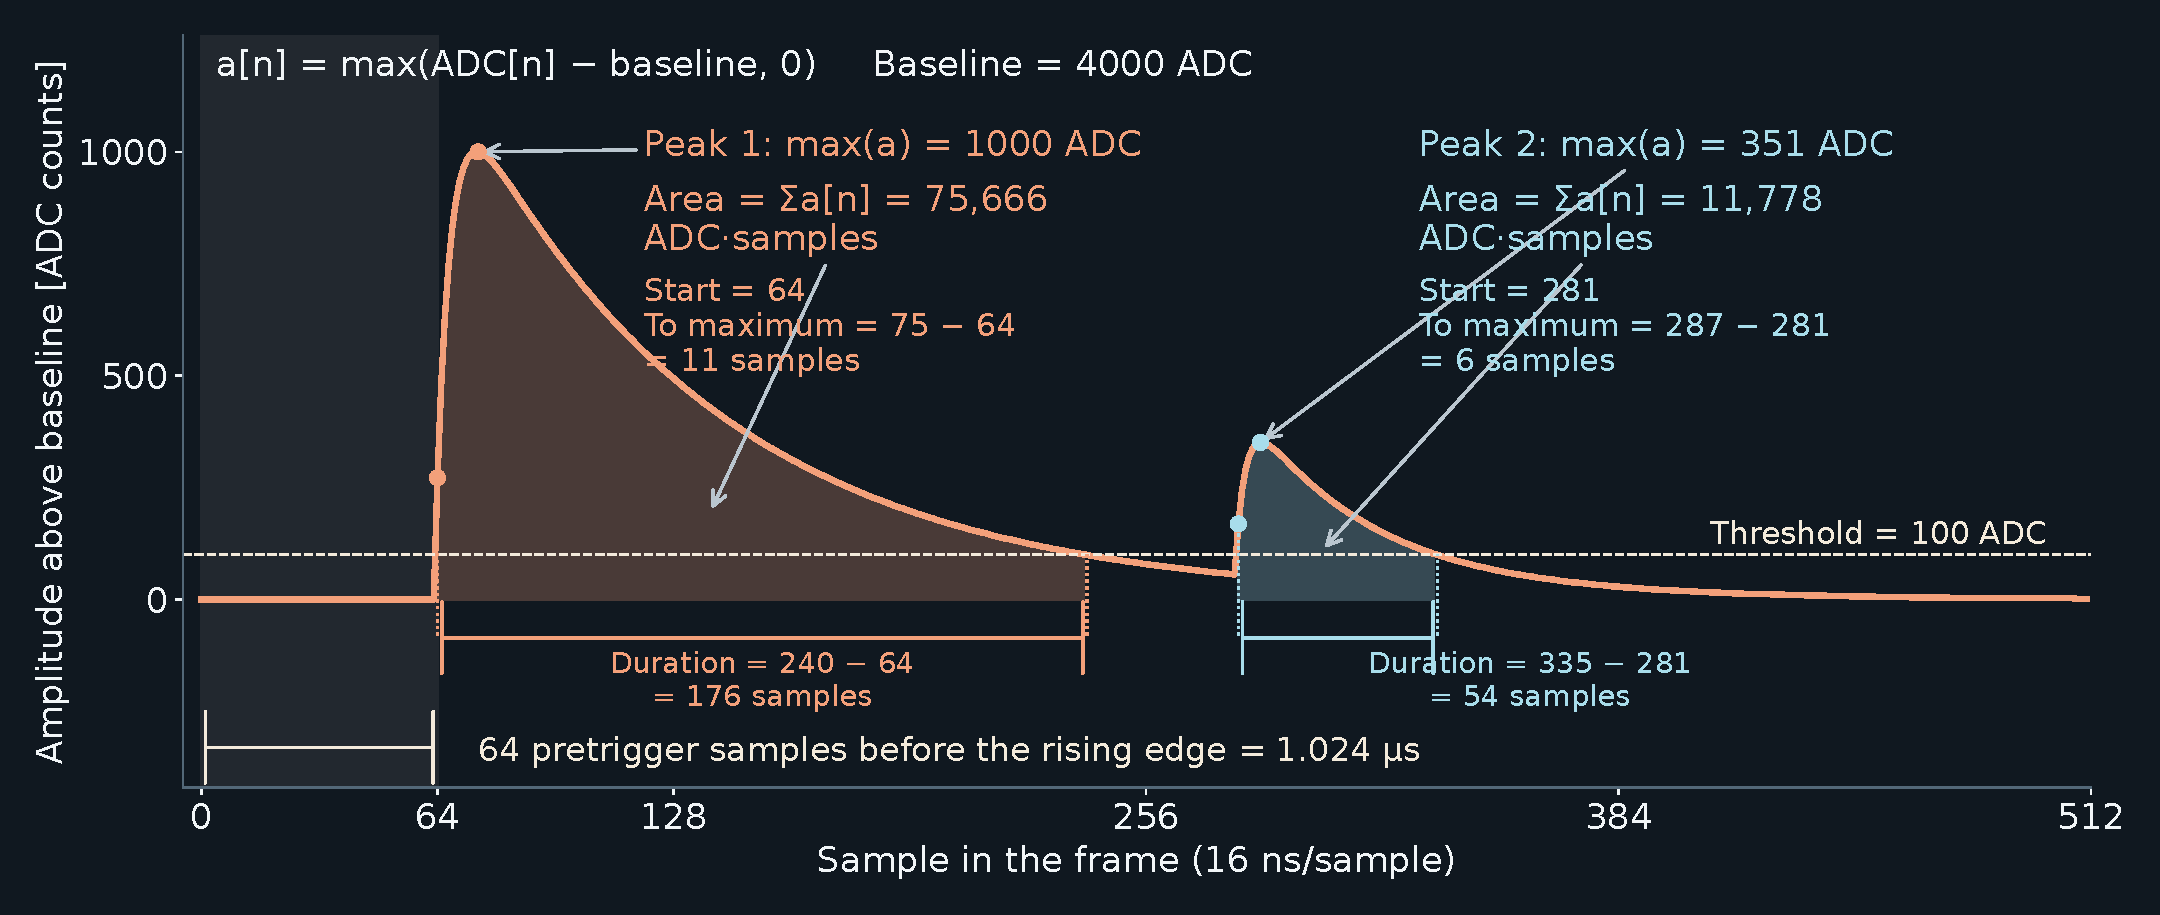
\includegraphics[width=\textwidth,height=0.70\textheight,keepaspectratio]{figures/descriptor-time.pdf}\par
  \DuneDiagramCaption{Sum amplitudes above threshold; do not subtract the threshold. Both slots valid; format byte 0xF1. Illustrative waveform.}
\end{frame}

\begin{frame}{Five peak descriptors now cover half the waveform}
  \centering
  \begin{tikzpicture}[x=1cm,y=1cm]
    \node[text=DuneText,anchor=east] at (0.0,2.6) {1024 samples};
    \node[text=DuneText,anchor=east] at (0.0,0.9) {512 samples};
    \draw[DunePaper,line width=1.2pt] (0.3,2.1) rectangle (10.3,3.1);
    \node[text=DunePaper] at (5.3,2.6) {One waveform: up to 5 peak descriptors};
    \draw[DuneEditorialAccent,line width=1.5pt] (0.3,0.4) rectangle (5.3,1.4);
    \draw[DuneSky,line width=1.5pt] (5.3,0.4) rectangle (10.3,1.4);
    \node[text=DuneEditorialAccent,align=center] at (2.8,0.9) {First 512 samples\\up to 5 descriptors};
    \node[text=DuneSky,align=center] at (7.8,0.9) {Next 512 samples\\up to 5 descriptors};
    \foreach \x/\label in {0.3/0,5.3/512,10.3/1024} {
      \node[text=DuneTextMuted,anchor=north] at (\x,0.15) {\label};
    }
  \end{tikzpicture}\par
  \DuneDiagramCaption{The same five-peak format gives finer descriptor coverage: up to ten peak summaries over 1024 samples when both fragments are retained.}
\end{frame}

% Generated by render_results.py; edit the generator, not this file.
\begin{frame}{Every common packet matches}
  \framesubtitle{Fresh five-mode RTL replay; firmware 7a25777e}
  \small
  \renewcommand{\arraystretch}{1.3}
  \begin{tabular}{@{}lrrrr@{}}
    \toprule
    Mode & Grouped packets & Native packets & Common / identical & Max latency [$\mu$s] \\
    \midrule
    0 & 3,392 & 3,392 & 3,392 & 17.984 \\
    1 & 3,372 & 3,372 & 3,372 & 17.952 \\
    2 & 2,224 & 2,200 & 2,200 & 560.432 \\
    3 & 3,672 & 3,446 & 944 & 48.272 \\
    4 & 3,296 & 3,272 & 3,272 & 17.984 \\
    \bottomrule
  \end{tabular}\par
  \medskip
  13,180 common packets are byte-identical; 16,198,656 ADC samples checked across both implementations.\par\medskip
  Mode 4 includes deliberate reset and disable losses. Latency runs from the first sample to the final output word.
\end{frame}


\begin{frame}{Count saved samples, not just packets}
  \centering
  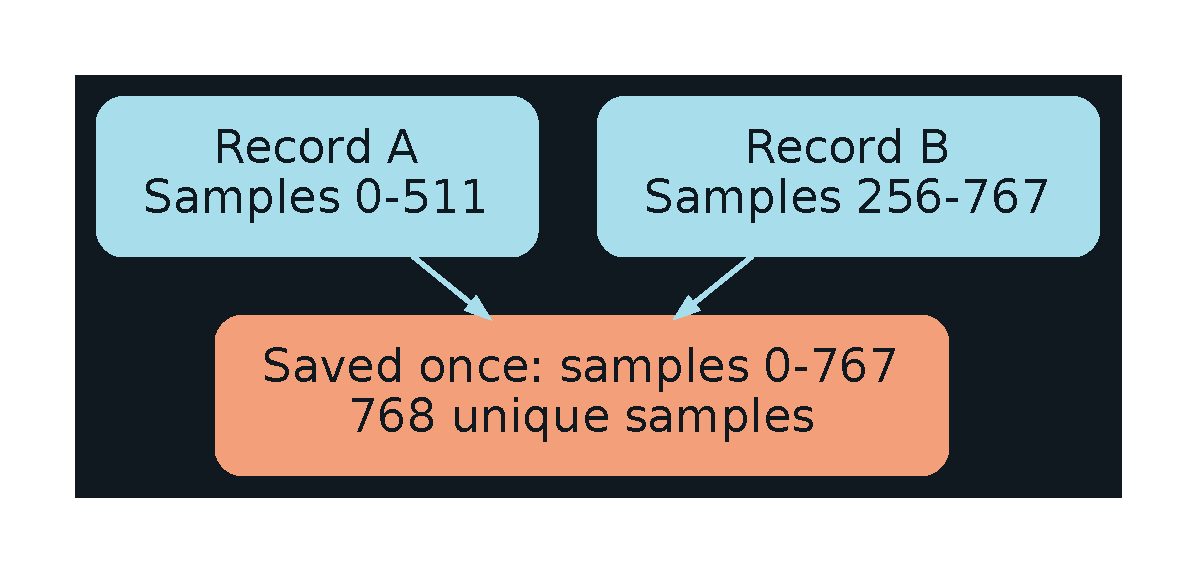
\includegraphics[width=0.91\textwidth,height=0.62\textheight,keepaspectratio]{diagrams/coverage.pdf}\par
  \DuneDiagramCaption{Merge overlapping windows before measuring loss. Each nonzero input sample counts once; quiet samples are outside the denominator.}
\end{frame}

\begin{frame}{Stop the output and watch what happens}
  \DuneBigStatement{ONE STRESS TEST}{Pause all lanes for 544 microseconds.}
    {Let the buffers fill. Restart readout. Check what was kept, what was lost, and whether it recovers.}
  \DuneDiagramCaption{Other cases check simultaneous pulses, short stalls, overlapping triggers, and reset.}
\end{frame}

\begin{frame}{Eight lanes feed four links}
  \centering
  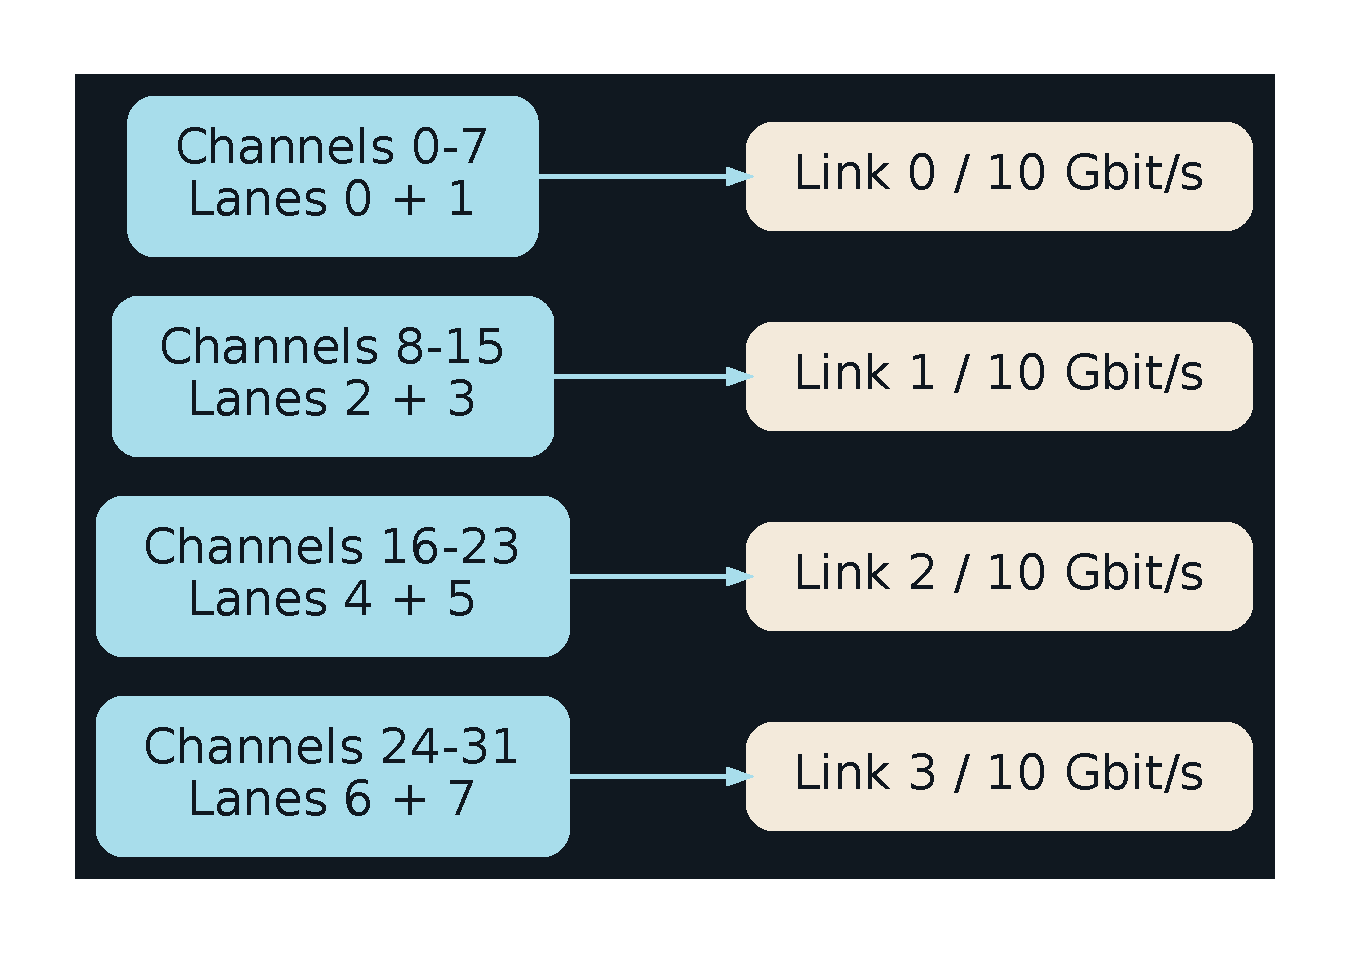
\includegraphics[width=0.90\textwidth,height=0.68\textheight,keepaspectratio]{diagrams/links.pdf}\par
  \DuneDiagramCaption{Grouped32 mapping. The replay checks the lanes; it does not send data through physical Ethernet.}
\end{frame}

\begin{frame}{Full stream also pairs two streams per link}
  \centering
  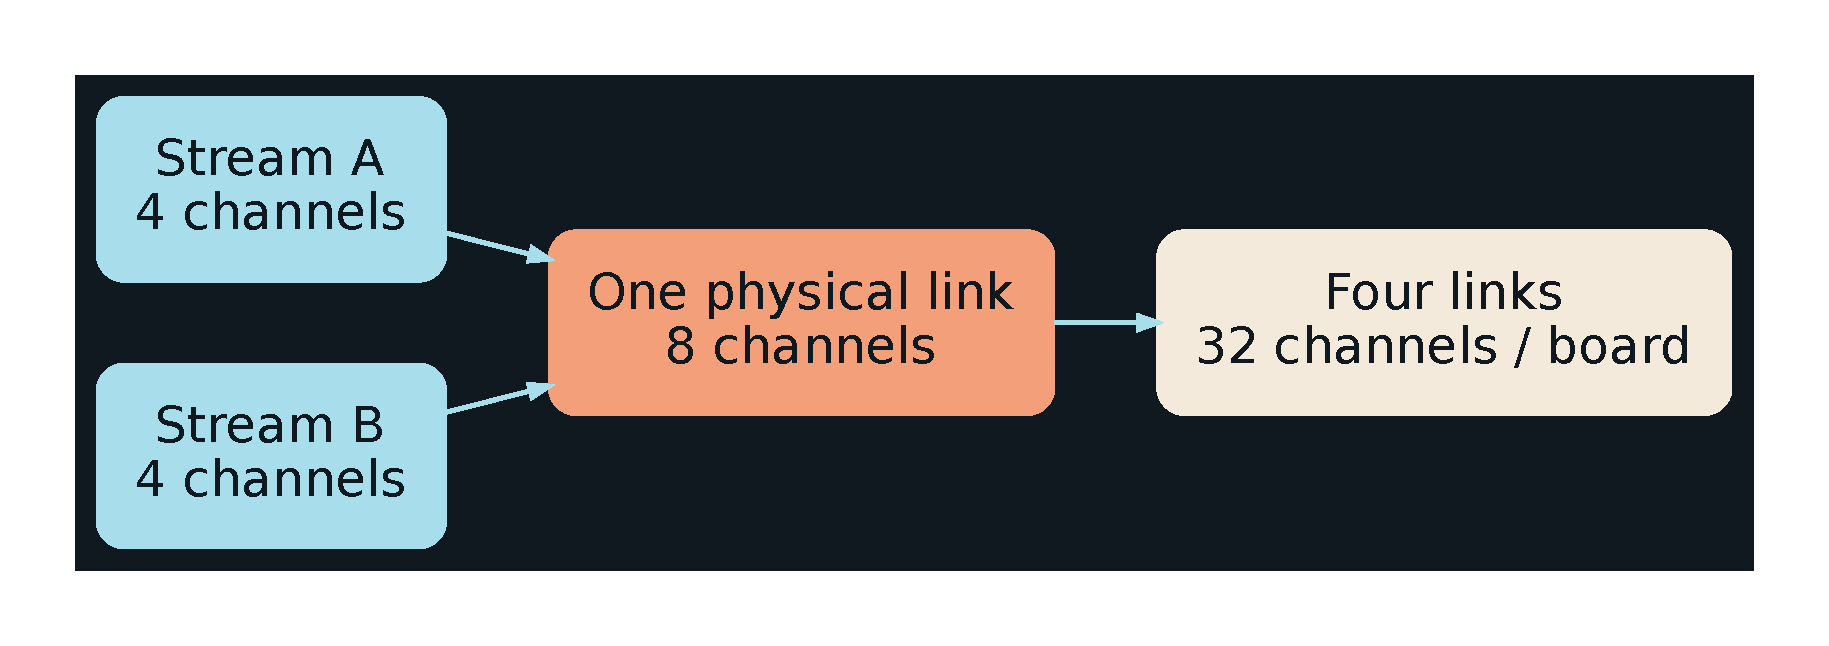
\includegraphics[width=\textwidth,height=0.64\textheight,keepaspectratio]{diagrams/fullstream-mapping.pdf}\par
  \DuneDiagramCaption{Checked full-stream source: four channels per logical stream, eight per physical link, 32 per board. Installed image and channel selection were not checked.}
\end{frame}

\begin{frame}{Expected traffic from the modeled activity only}
  \centering
  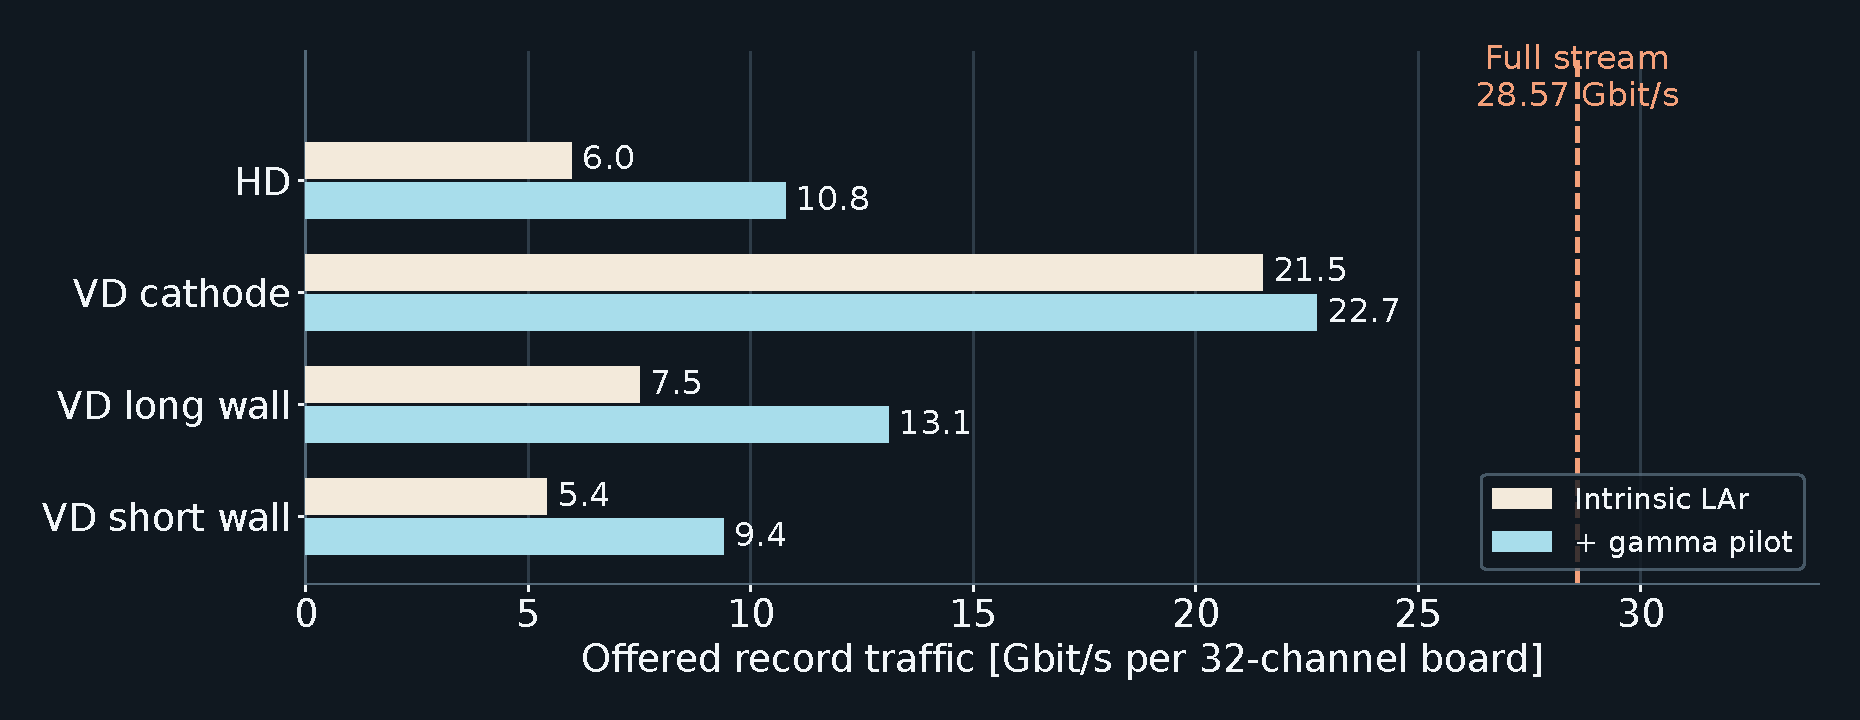
\includegraphics[width=\textwidth,height=0.68\textheight,keepaspectratio]{figures/traffic.pdf}\par
  \DuneDiagramCaption{Other background sources are not included. 32 channels; one self-trigger record per candidate, before losses or continuation. Both estimates exclude network overhead.}
\end{frame}

\begin{frame}{Full stream is constant; self-trigger follows activity}
  \centering
  \renewcommand{\arraystretch}{1.5}
  \begin{tabular}{@{}lll@{}}
    \toprule
    Same 32-channel board & Full stream & Self-trigger 512 + ring \\
    \midrule
    What is sent? & Every sample & Selected windows + peaks \\
    What sets the rate? & ADC sample clock & Saved records per second \\
    HD example below & 28.57 Gbit/s & 10.78 Gbit/s \\
    \bottomrule
  \end{tabular}\par\medskip
  HD intrinsic + gamma pilot: 43,855 candidates/s/channel.\par\smallskip
  $32\times43{,}855\times960\ \mathrm{bytes}\times8
     =10.78\ \mathrm{Gbit/s}$.\par\medskip
  \DuneDiagramCaption{Estimate: one 512-sample record per candidate; no continuation, merging, or losses modeled. Other backgrounds are excluded. Both rates include record headers, not network overhead.}
\end{frame}

\begin{frame}{Preprocessing matters even when traffic stays high}
  \DuneBigStatement{CONTINUOUS ACTIVITY}{The descriptors still save pulse-finding work.}
    {Continuous self-trigger records reach 30 Gbit/s for 32 channels. Bandwidth savings can disappear while the preprocessing benefit remains.}
\end{frame}

\begin{frame}{The LArSoft numbers are a dated snapshot}
  \small
  \begin{tabular}{@{}ll@{}}
  \toprule
  Software & dunesw v10\_22\_00d01; larsoft v10\_22\_00 \\
  Detector models & FD horizontal drift (HD), vertical drift (VD) \\
  Candidate selection & Above 0.7 photoelectrons (PE); no 10 MeV cut \\
  Intrinsic baseline & Atmospheric argon mixture; eight shards \\
  Gamma addition & One physical window per source family \\
  Snapshot & 9 September 2026; reused here, not rerun \\
  \bottomrule
  \end{tabular}\par\medskip
  Shared transport, a complete background inventory, and calibrated noise are still needed for a detector trigger prediction.
\end{frame}

\begin{frame}{Keep the result tied to its inputs}
  \small
  \textbf{Firmware:} \texttt{7a25777e}, grouped32 branch.\par\medskip
  \textbf{Run:} \texttt{scripts/run\_grouped32\_rtl\_study.py --run}.\par\medskip
  \textbf{Evidence:} this deck's README, JSON reports, CSV tables, and figure scripts.\par\medskip
  Behavioral memory and clock-crossing models; no physical Ethernet or analog capture test.
  \DuneSourceLine{Firmware architecture and verification}{\firmwaresource/docs/reports/grouped32/approval-review-20260915.md}
\end{frame}
